%!TEX program = xelatex
\documentclass[11pt]{article}
\usepackage{amssymb,amsfonts,amsthm,amsmath,bm,microtype}
\usepackage[left=21mm,text={148mm,200mm},paperwidth=185mm,paperheight=250mm,includehead,vmarginratio=1:1]{geometry}
\usepackage[all]{xy}
\usepackage{tikz}
\usepackage{titletoc}%使用目录
	\theoremstyle{plain}%定理环境样式
	\newtheorem{pro}{Proposition}[section]% 定义命题环境
	%\newtheorem{theo}{Theorem}[section]% 定义定理环境
	%\newtheorem{lem}{Lemma}[section]% 定义引理环境
	\newtheorem*{rem}{Remark}% 定义注记环境
	\newtheorem{que}{Question}[section]% 定义问题环境
	\newtheorem{defi}{Definition}[section]% 定义定义环境
	\newtheorem{exa}{Example}[section]% 定义例子环境
	%\newtheorem{exe}{Exercise}[section]% 定义习题环境

\usepackage{hyperref}  % 使用xetex引擎
	\hypersetup  % 一些选项
{
	pdftoolbar=true,  % 显示Acrobat工具栏
	pdfmenubar=true,  % 展开Acrobat目录
	pdftitle={Bundle},  % pdf题目,自己填
	pdfauthor={Unsinn},  % pdf作者,自己填
	bookmarksnumbered=true,  % 书签中章节编号
	bookmarksopen=true,  % 目录层次打开
	bookmarksopenlevel=1,  % 目录层次打开的级数,可选数字或者 \maxdimen最大
	pdfsubject={Mathematics},  % 主题,自己填
	pdfkeywords={Bundle},  % 关键字,自己填
	colorlinks=true,  % 彩色链接 false:边框链接 ; true: 彩色链接
	linkcolor=blue,  % 内部链接颜色
	citecolor=green,  % 引用标记颜色
	filecolor=magenta,  % 文件链接颜色
	urlcolor=cyan  % URL链接颜色
}

%定义你的命令
\newcommand{\dd}{{\mathrm{d}}}  % 微分号
\newcommand{\no}[1]{{$(#1)$}}  % 编号
\newcommand{\rr}{{\mathbb{R}}}  % 实数域
\newcommand{\cc}{{\mathbb{C}}}  % 复数域
\newcommand{\lag}{{\mathfrak{g}}}  % Lie代数
\newcommand{\ad}{{\mathrm{ad}}}
\definecolor{shadecolor}{rgb}{0.92,0.92,0.92}
\newcommand{\re}[1]
	{\begin{center}
		\colorbox{shadecolor}{
			\begin{minipage}{135mm}
				\emph{''#1''}
			\end{minipage}}
	\end{center}}

\begin{document}
\section{Section}
\subsection{Foundation}
A fiber bundle is a structure $(E, B, \pi, F)$, where $E$, $B$, and $F$ are topological spaces and $\pi : E \rightarrow B$ is a continuous surjection satisfying a local triviality condition outlined below. The space $B$ is called the base space of the bundle, $E$ the total space, and $F$ the fiber. The map $\pi$ is called the projection map (or bundle projection). We shall assume in what follows that the base space $B$ is connected.

We require that for every $x$ in $E$, there is an open neighborhood $U \subset B$ of $\pi(p)$ (which will be called a trivializing neighborhood) such that there is a homeomorphism $\varphi : \pi^{-1}(U) \rightarrow U \times F$ (where $U \times F$ is the product space) in such a way that $\pi$ agrees with the projection onto the first factor. That is, the following diagram should commute:
\begin{figure}[htp]
	\centering
	\[
		\xymatrix{
			\pi^{-1}\left(U\right)\ar[rr]^\varphi \ar[dr]_\pi&&U\times F \ar[dl]^{\mathrm{proj}_1}\\
			&U&
			}
	\]
	\caption{Locally Trivialition}
\end{figure}
 where $\mathrm{proj}_1 :U \times F\rightarrow U$ is the natural projection and $\varphi : \pi^{-1}(U) \rightarrow U \times F$ is a homeomorphism. The set of all ${(U_i, \varphi_i)}$ is called a local trivialization of the bundle. Especially, if $F$ and every $\pi^{-1}(p)$ are vector spaces, we call this bundle vector bundle.
\begin{defi}
	A section $s$ on a bundle $(E,M,\pi,F)$ is a map $s:M\rightarrow E$ such that $\pi\circ s=\mathrm{Id}_E$.
\end{defi}
Here's the trivial bundle $E=M \times F$ and a section on it:
\begin{figure}[htp]
\centering
	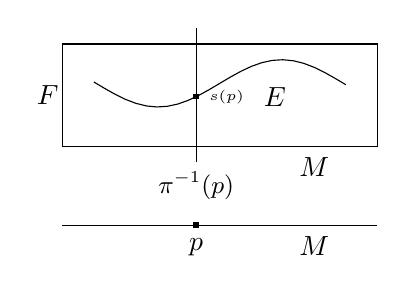
\begin{tikzpicture}[scale=1]
		\draw (-2,-0.3)--(2,-0.3)--(2,1)--(-2,1)--cycle;
		\node [label=left:$F$] (F) at (-1.8,0.35) {};
		\node [label=below:$M$] (M1) at (1.2,-0.2) {};
		\node [label=below:$M$] (M2) at (1.2,-1.2) {};
		\node [label=below:$E$] (E) at (0.7,0.7) {};
		\draw (-2,-1.3)--(2,-1.3);
		\node [fill=black, inner sep=1pt, label=below:$p$] (p) at (-0.3,-1.3) {};
		\draw [color=black, domain=-1.6:1.6] plot (\x,{0.3*sin(2*\x r)+0.5});
		%0.5-0.3*sin(0.6)=0.330607...
		\node [fill=black, inner sep=1pt, label=right:\tiny$s(p)$] (s) at (-0.3,0.3306) {};
		\draw (-0.3,-0.5)node[below]{\small$\pi^{-1}(p)$}--(-0.3,1.2);
	\end{tikzpicture}
	\caption{Trivial Bundle and its Section}
\end{figure}

For every $p\in M$, $s(p)\in \pi^{-1}(p) \cong F$, thus $s(p)$ is like an element in $F$. If $E$ is a vector bundle, $s(p)$ correspond to a vector in $F$ and $s$ play the role of a \textit{vector field} on $M$. Naturally, we will have the definition below.
\begin{defi}
	A vector field on a manifold $M$ is a section of vector bundle $(E,M,\pi,F)$.
\end{defi}
Sections have the linear structure inherited from $F$:
\[
	\begin{split}
		&(s_1+s_2)(p)=s_1(p)+s_2(p),\\
		&(fs)(p)=f(p)s(p),
	\end{split}
\]
where $f$ is a real-valued function on $M$.

For any vector space $V$, $L(V)$ is also a vector space, and so we can have another vector bundle $(E',M,\pi,L(F))$ and its section $T:M\rightarrow E'$. In vector space, it's very important for us to research the linear map acting on a vector. The analogous research here is the section fo $E'$ acting on a section of $E$. We can define it by $T(s)(p)=T(p)s(p)$, and it should have
\[
	T(s_1+s_2)=T(s_1)+T(s_2) \text{\ and\ } T(fs)=fT(s).
\]
From now on, we will use $\Gamma(E)$ to denote the set of all sections on bundle $E$ and $\mathrm{End}(E)$ to replace $E'$ used above.
\begin{exa}
	Tangent bundle and Cotangent bundle:

	The tangent bundle of a differentiable manifold $M$ is the disjoint union of the tangent spaces of $M$.
	\[
		TM =\coprod_{x\in M}T_xM=\bigcup_{x\in M} \left\{x\right\}\times T_xM
		=\bigcup_{x\in M} \left\{(x, y)\vert\; y\in T_xM\right\}.
	\]
	where $T_xM$ denotes the tangent space to $M$ at the point $x$. So, an element of $TM$ can be thought of as a pair $(x, v)$, where $x$ is a point in $M$ and $v$ is a tangent vector to $M$ at $x$.There is a natural projection 
	\[
		\pi : TM \rightarrow M 
	\]
	defined by $\pi(x, v) = x$. This projection maps each tangent space $T_xM$ to the single point $x$.

	Similarly, the cotangent bundle $T^*\!M$ is the vector bundle of all the cotangent spaces at every point in the manifold.
\end{exa}
\subsection{Vector-valued Form on $M$}
Let's start from the vector-valued 1-form. 

A (real-valued) 1-from $\omega:TM\rightarrow \mathbb{R}$ is in $T^*\!M$. Now suppose we have a topological space $E$, a $E$-valued 1-form on $p \in M$ is locallly defined by
\[
	v(p)\otimes\omega(\dot{p}):T_pM\rightarrow E\otimes \mathbb{R},
\]
where $v(p)\in E$ and $\dot{p} \in T_p M$, and thus globally $v\otimes\omega:TM\rightarrow E\otimes \mathbb{R}$.

\subsection{The geometry of the tangent bundle}
Tangent bundle is also a manifold, so it's natural to talk about its tangent bundle. Suppose there are a manifold $Q$, tangent bundle $TQ$ and its tangent bundle $TTQ$. Introducing the local coordinates $(q^i)$ in $Q$, $(q^i,v^i)$ in $TQ$ and $(q^i,v^i,\dot{q}^i,\dot{v}^i)$ in $TTQ$, we can write their elements $v \in T_qQ$ and $V \in T_vTQ$ locally as
\[
	v=v^i\frac{\partial}{\partial q^i} \quad\text{and}\quad V=\dot{q}^i\frac{\partial}{\partial q^i}+\dot{v}^i\frac{\partial}{\partial v^i},
\]
and the natural projections
\[
	\pi_Q(q^i,v^i)=(q^i),\quad \pi_{TQ}(q^i,v^i,\dot{q}^i,\dot{v}^i)=(q^i,v^i)\quad\text{and}\quad \left(\pi_{Q}\right)_*(q^i,v^i,\dot{q}^i,\dot{v}^i)=(q^i,\dot{q}^i).
\]
These can be shown by the diagram:
\begin{figure}[htbp]
	\centering
	\[
		\xymatrix{
			TTQ\ar[rr]^{\left(\pi_{Q}\right)_*} \ar[d]^{\pi_{TQ}}&&TQ\ar[d]_{\pi_{Q}}\\
			TQ\ar[rr]^{\pi_{Q}} &&Q
			}
	\]
	\caption{The Natural Projections}
\end{figure}
\begin{defi}
	Vertical fiber bundle $\ker(\pi_Q)_*$ is the disjoint union of the kernal of $(\pi_Q)_{*v}$ at each point $v$ of $TTQ$.
\end{defi}
\begin{defi}
	Let $v \in T_qQ$ be vector tangent to $Q$ at some point $q\in Q$, the vertical lift of $v$ at a point $w\in T_qQ$ is the tangent vector $\mathrm{Vert}_w(v)\in T_wTQ$ given by
	\[
		\mathrm{Vert}_w(v)f=\left.\frac{\dd}{\dd t}f(w+tv)\right|_{t=0},\quad \forall f\in \mathcal{C}^\infty(T_qQ).
	\]
\end{defi}

Given a smooth function $f\in \mathcal{C}^\infty(Q)$,
\[
	\begin{split}
		(\pi_Q)_{*w}\mathrm{Vert}_w(v)(f)&=\mathrm{Vert}_w(v)(f\circ \pi_Q)\\
		&=\left.\frac{\dd}{\dd t}f(\pi_Q(w+tv))\right|_{t=0}\\
		&=\left.\frac{\dd}{\dd t}f(q)\right|_{t=0}=0.
	\end{split}
\]
Thus $\mathrm{Vert}_w$ takes value in a fiber of vertical fiber bundle:
\[
	\mathrm{Vert}_w:T_qQ\to\ker(\pi_Q)_{*w}\subset T_wTQ.
\]
Indeed, for each $w \in T_q Q$, the vertical lift $\mathrm{Vert}_w$ is a linear isomorphism between $T_q Q$ and $\ker(\pi_Q)_{*w}$. Using local coordinates, if $v=(q^i,v^i)$ and $w=(q^i,w^i)$, then
\[
	\mathrm{Vert}_w(v)=(q^i,w^i,0,v^i).
\]
\begin{defi}
	The vertical endomorphism is the linear map $\mathcal{S}:TTQ\to TTQ$ that, ofr any vector $V \in TTQ$, gives the value
	\[
		\mathcal{S}(V)=\mathrm{Vert}_v\left(\left(\pi_Q\right)_{*v}V\right),
	\]
	where $v=\pi_{TQ}V\in TQ$.
\end{defi}
\begin{defi}
	The Liouville or dilation vector field is the vector field $\Delta$ over $TQ$ defined by
	\[
		\Delta_v=\mathrm{Vert}_v(v).
	\]
\end{defi}

In adapted coordinates $(q^i,v^i)$ of $T Q$ , the vertical endomorphism has the local expression 
\[
	\mathcal{S}(q^i,v^i,\dot{q}^i,\dot{v}^i)=(q^i,v^i,0,\dot{q}^i)=\dd q^i\otimes\frac{\partial}{\partial v^i},
\]
the second equality is valid because
\[
	\left\langle \dd q^i,\dot{q}^i\frac{\partial}{\partial q^i}+\dot{v}^i\frac{\partial}{\partial v^i}\right\rangle\frac{\partial}{\partial v^i}=\dot{q}^i\frac{\partial}{\partial v^i},
\]
and the Liouville vector field is 
\[
	\Delta=(q^i,v^i,0,v^i)=v^i\frac{\partial}{\partial v^i}.
\]
Another way to define the Liouville vector field is as the infinitesimal generator of the 1-parameter group of transformations $\phi_t : v \in T Q \mapsto e^t v \in T Q$, that is, if $v=(q^i,v^i)$, then $\phi_t : v  \mapsto (q^i,e^tv^i)\in T Q$, and
\[
	\left.\frac{\dd}{\dd t}\phi_tv\right|_{t=0}=(q^i,e^tv^i,0,e^tv^i)_{t=0}=(q^i,v^i,0,v^i).
\]
This definition can easily be translated to any vector bundle.
\begin{defi}
	A second order vector field $X$ is a section of $TTQ$ such that $(\pi_Q)_*\circ X=\mathrm{Id}_{TQ}$.
\end{defi}
This mean that $(\pi_Q)_*\circ X=\pi_{TQ}\circ X$, so a second order vector field is well defined. In adapted coordinates $(q^i,v^i)$ of $T Q$ , $X$ is a vector field
\[
	X = (q^i,v^i,v^i,a^i),
\]
where $(a^i)$ is arbitrary. Thus, neither the Liouville vector field nor the vertical lift of a vector field are second
order vector fields. Even though, second order vector fields are characterized by the equation
\[
	\mathcal{S}(X)=\Delta,
\]
locally, it is
\[
	\mathcal{S}(q^i,v^i,v^i,w^i)=(q^i,v^i,0,v^i)=\Delta.
\]

\begin{defi}
	Given a smooth curve $c:I\to Q$, its (first) lift to $TQ$ is the smooth curve $c^{(1)}:I\to TQ$ such that
	\[
		c^{(1)} (t_0)f=\left.\frac{\dd}{\dd t}(f\circ c)\right|_{t=t_0}.
	\]
\end{defi}
In local adapted coordinates
\[
	c^{(1)}=(c^i,\dd c^i/\dd t).
\]
\begin{pro}
	A vector field $X \in \Gamma(TTQ)$ is a second order vector field if and only if the integral curves of $X$ are lifts of their own projections to $Q$; that is, if $\widetilde{c}$ is an integral curve of $X$, then
	\[
		\widetilde{c}=(\pi_Q\circ \widetilde{c})^{(1)}.
	\]
	The curve $c=\pi_Q\circ \widetilde{c}:I\to Q$ is called a base integral curve of X or a solution of the second order differential equation given by X.
\end{pro}
If $\widetilde{c}:I \to TQ$ is an integral curve of a second order vector field $X \in \Gamma(TTQ)$ locally given by $X=(q^i,v^i,v^i,a^i)$ and $c:I \to Q$ denotes its base integral curve, then
\[
	q^i=c^i,\quad v^i=\dot{c}^i\quad\text{and}\quad a^i=\ddot{c}^i.
\]
Alternatively, the base integral curve $c$ of $\widetilde{c}$ satisfies the system of second order differential quations
\[
	\ddot{c}^i = a^i (c^i , \dot{c}^i).
\]

\end{document}